\clearpage
\subsection{C String} % (fold)
\label{sub:c_string}

C was designed to build for use with the Unix operating system. When the language was designed string manipulation was not a high priority, and therefore C does not have built in capabilities to perform tasks like concatenating strings, and copying strings (i.e. assigning a string a value after it has been declared).

Working with c-strings requires that you think about how the text is represented in the computer. \tref{tbl:c-string-fred} shows the characters used to store the text value `Fred'. 

As C does not keep the length of the array there needs to be a means of determining how long the string is. The method that C choose was to place a \textbf{sentinel} value at the end of the string. This marks the position in the array where the string ends. The sentinel is the \texttt{null} character, the one with value the \texttt{0}.

\begin{table}[h]
\begin{minipage}{\textwidth}
  \centering
\begin{tabular}{|l|c|c|c|c|c|}
\hline
Characters: & F & r & e & d & \texttt{\textbackslash 0} \\
\hline
Bytes Values\footnote{Byte values are shown as decimal.}: & \texttt{70} & \texttt{114} & \texttt{101} & \texttt{100} & \texttt{0} \\
\hline
\end{tabular}
\caption{The characters and byte values for the c-string containing the text `Fred'}
\label{tbl:c-string-fred}
\end{minipage}
\end{table}

Space characters are distinct from the \texttt{null} character. \tref{tbl:c-string-fred-smith} shows the characters involved in storing the text `Fred Smith'. The space character is the value 32, and the sentinel value only appears at the end of the c-string. To store `Fred Smith' you need an array that can store at least 11 characters. Ten for the characters in the name, and one for the sentinel.

\begin{table}[h]
\begin{minipage}{\textwidth}
  \centering
\begin{tabular}{|l|c|c|c|c|c|c|c|c|c|c|c|c|}
\hline
Characters: & F & r & e & d &  & S & m & i & t & h & \texttt{\textbackslash 0}\\
\hline
Bytes Values\footnote{Byte values are shown as decimal.}: & \texttt{70} & \texttt{114} & \texttt{101} & \texttt{100} & \texttt{32} & \texttt{83} &\texttt{109} & \texttt{105} & \texttt{116} & \texttt{104} & \texttt{0} \\
\hline
\end{tabular}
\caption{Characters for `Fred Smith', the space has the character value 32.}
\label{tbl:c-string-fred-smith}
\end{minipage}
\end{table}

It is possible for an array to have more characters that are needed. \tref{tbl:c-string-fred-null-smith} shows an array with 11 characters that is storing the c-string `Fred'. The \texttt{null} character at index 4 (the $5^{th}$ character) ends the c-string and the remainder of the data in the array will be ignored by the c-string functions.

\begin{table}[h]
\begin{minipage}{\textwidth}
  \centering
\begin{tabular}{|l|c|c|c|c|c|c|c|c|c|c|c|c|}
\hline
Characters: & F & r & e & d & \texttt{\textbackslash 0} & S & m & i & t & h & \texttt{\textbackslash 0}\\
\hline
Bytes Values\footnote{Byte values are shown as decimal.}: & \texttt{70} & \texttt{114} & \texttt{101} & \texttt{100} & \texttt{0} & \texttt{83} &\texttt{109} & \texttt{105} & \texttt{116} & \texttt{104} & \texttt{0} \\
\hline
\end{tabular}
\caption{This would only print `Fred', as the 0 character indicates the end of the c-string}
\label{tbl:c-string-fred-null-smith}
\end{minipage}
\end{table}

The code in \lref{clst:test-strings} shows some examples of the main operations you may want to perform on strings. This includes the following actions:
\begin{itemize}
  \item \textbf{Initialisation}: Creating and initialising a string.
  \item \textbf{Input}: Reading words, and lines, from the Terminal.
  \item \textbf{Comparison}: Checking if two strings are equal. Notice that you also need to check the \texttt{null} value.
\end{itemize}
Other common string operations are found in \lref{clst:populate_array}. These included:
\begin{itemize}
  \item \textbf{Copy}: Assigning one string to another, as you cannot use the assignment statement to achieve this in C.
  \item \textbf{Concatenate}: Adding one string to the end of another.
\end{itemize}

\csection{\ccode{clst:test-strings}{Code illustrating working with Strings in C}{code/c/array/test-string.c}}

\mynote{
\begin{itemize}
  \item In C a String is an array of characters. There is little built in support beyond this in the C language itself. The Standard C libraries include functions that can be used to work with String data, in \texttt{strings.h}.
  \item \textbf{Remember} to ask for enough space to store the text and the sentinel value when declaring a c-string. If you want to store 4 characters then you need to ask for an array with space for 5, the 4 characters + and 1 sentinel value.
  \item The c-string functions will look for the null character. If the null character is missing from the end of the c-string then these functions will not work as you want. The problem is that they may appear to be working, though in reality they are interacting with memory that is not associated with the c-string you are working on.
  \item \textbf{Take care when working with c-strings!} Many security issues in software relate to incorrect handling of c-strings.
\end{itemize}
}

\clearpage

\subsubsection{Print and Scanning in Strings} % (fold)
\label{ssub:print_and_scanning_in_strings}

The \texttt{stdio.h} header also provides version of \texttt{printf} and \texttt{scanf} that are used to write values to, and read values from strings. The \texttt{sprintf} function writes data into a \texttt{destination} string, whereas the \texttt{sscanf} function reads data out of a source \texttt{string}. \tref{tbl:sprintf} shows the details for the \texttt{sprintf} function, \tref{tbl:sscanf} shows the details for \texttt{sscanf}.

\begin{table}[h]
  \centering
  \begin{tabular}{|c|p{9cm}|}
    \hline
    \multicolumn{2}{|c|}{\textbf{Function Prototype}} \\
    \hline
    \multicolumn{2}{|c|}{} \\
    \multicolumn{2}{|c|}{\texttt{int sprintf(char *destination, const char *format, \ldots )}} \\
    \multicolumn{2}{|c|}{} \\
    \hline
    \multicolumn{2}{|c|}{\textbf{Returns}} \\
    \hline
    \texttt{int} & The number of characters written to the \texttt{destination} by \texttt{sprintf}. \\
    \hline
    \textbf{Parameter} & \textbf{Description} \\
    \hline
    \texttt{ destination } & The string to write the output into. \textbf{Warning:} You are responsible for ensuring there is enough space.\\
    & \\
    \texttt{ format } & The text that is to be written to the Terminal. This text may contain format tags to include other values. This is the same as \texttt{printf}, see Figure \ref{csynt:program-creation-format-string} for the syntax of the format tag. \\
    & \\
    \texttt{\ldots}   & Optional values, must have at least as many values as format tags. \\
    \hline
  \end{tabular}
  \caption{Parameters that must be passed to \texttt{sprintf}}
  \label{tbl:sprintf}
\end{table}


\begin{table}[h]
  \centering
  \begin{tabular}{|c|p{9.5cm}|}
    \hline
    \multicolumn{2}{|c|}{\textbf{Function Prototype}} \\
    \hline
    \multicolumn{2}{|c|}{} \\
    \multicolumn{2}{|c|}{\texttt{int sscanf(const char *source, const char *format, \ldots )}} \\
    \multicolumn{2}{|c|}{} \\
    \hline
    \multicolumn{2}{|c|}{\textbf{Returns}} \\
    \hline
    \texttt{int} & The number of values read by \texttt{sscanf}. \\
    \hline
    \textbf{Parameter} & \textbf{Description} \\
    \hline
    \texttt{ source } & The string from which the input is read.\\
    & \\
    \texttt{ format } & The format specifier describing what is to be read from the Terminal. This is the same as with \texttt{scanf}, see \tref{tbl:format specifiers}. \\
    & \\
    \texttt{\ldots}   & The variables into which the values will be read. There must be at least as many variables as format tags in the format specifier. \\
    \hline
  \end{tabular}
  \caption{Parameters that must be passed to \texttt{sscanf}}
  \label{tbl:sscanf}
\end{table}

\mynote{
\begin{itemize}
  \item These functions are useful for converting data to and from string values.
  \item You can use \texttt{sprintf} to convert numeric values and store them in a string. Though care must be taken to ensure that there is sufficient space for these values in the destination string.
  \item \texttt{sscanf} can be used to read values out of a string. For example, you could read a numeric value out of a string value entered by the user.
\end{itemize}
}



% subsubsection print_and_scanning_in_strings (end)

\clearpage
\subsubsection{Example use of C-string functions} % (fold)
\label{ssub:example_use_of_c_string_functions}

The Statistics Calculator requires some string manipulation to generate the prompt that will be shown to the user. The prompt is created from the text `\texttt{Enter value}', the value of \texttt{i + 1}, and the text `\texttt{: }'. The four function calls needed to achieve this are shown in \fref{fig:cstringops}.

\begin{figure}[htbp]
   \centering
   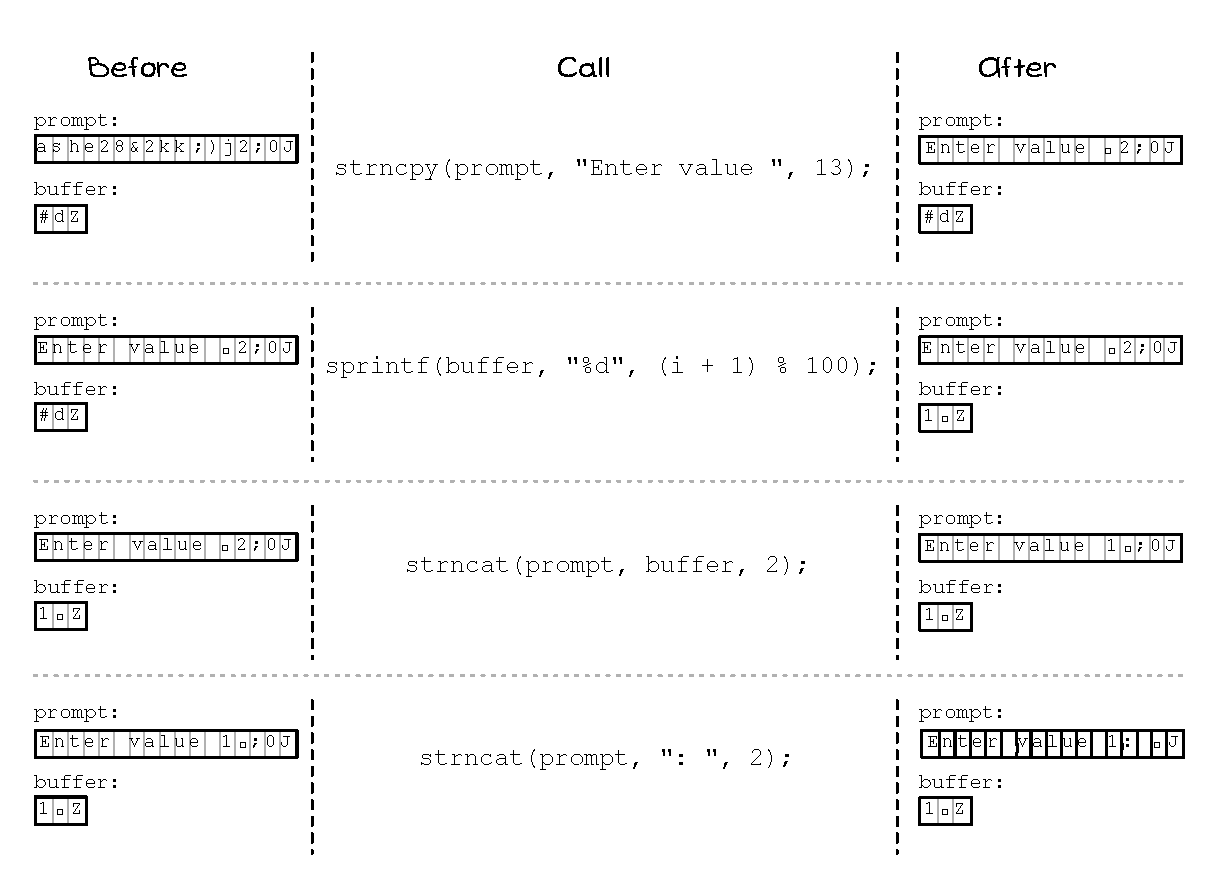
\includegraphics[width=\textwidth]{./topics/arrays/images/CStringOps} 
   \caption{Example usage of c-string functions from the Statistics Calculator}
   \label{fig:cstringops}
\end{figure}

\mynote{
\begin{itemize}
  \item The steps shown in \fref{fig:cstringops} perform the following actions:
  \begin{enumerate}
      \item The first instruction uses \texttt{strncpy} to copy the characters in `\texttt{Enter value}' into the \texttt{prompt}. The \texttt{null} character must also be copied so that \texttt{strncat} knows where the string currently ends.
      \item Step 2 uses \texttt{sprintf} to print the decimal value of \texttt{(i + 1) \% 100} into the \texttt{buffer}. This uses \texttt{\% 100} so that only two characters\footnote{\texttt{(i + 1) \% 100} is the remainder of the value i incremented by one after dividing by 100. This ensures that it is always between 0 and 99. For example, when \texttt{i} is 106, \texttt{i + 1} is 107, and \texttt{107 \% 100} is 7, the remainder of dividing 107 by 100.} and the terminal are ever written into the \texttt{buffer}. 
      This assumes that the value of \texttt{i} is 0, so \texttt{i + 1} is \texttt{1}.
      \item Next \texttt{strncat} is used to concatenate \texttt{prompt} and \texttt{buffer}. This copies the text in \texttt{buffer} to the end of \texttt{prompt}, and makes sure that there is a \texttt{null} character at the end. So the \texttt{n} in this case indicate the maximum number of actual characters to add to the destination, as the \texttt{null} is effectively moved in this function.
      \item The operation is completed by concatenating the final `\texttt{: }' to the end of the string.
  \end{enumerate}
  \item Notice that there is one additional character left in this \texttt{prompt} at the end, this gives space for two digit values, e.g. `\texttt{Enter value 10:}'.
\end{itemize}
}


% subsubsection example_use_of_c_string_functions (end)

% subsection c_string (end)